\section{Selection in practice: results from simulation}
\label{se:sec:simul}

We have undertaken simulation of our proposal regarding the energy consumption in order to compare it with the previous model (using pseudo-random election for \cns).
We used \ns software to proceed.

In the new proposal, the \vns are to model the theoretical consumption of the \cns they watch over.
We have chosen to use Rakhmatov and Vrudhula's diffusion model\cite{RV01} to compute the consumption.
This choice was driven by several reasons:
\begin{itemize}
    \item it provides a pretty accurate approximation of real consumption, taking into account chemical processes internal to the battery such as rate capacity effect and recovery effect;
    \item it is one of the models already implemented in \ns. So in our case it is an absolutely perfect theoretical model.
        It remains ``theoretical'' as \vns use this model to compute the expected behaviour of \cns according to the few packets they sometimes hear. Meanwhile, real \cns consumption computed by \ns core takes into account every packet actually sent or received by \cns, also including packets that \vns can not hear (because of distance or sleep schedule). So the values computed by \vns and \ns core will not always be the same, which allows us to use the model.
\end{itemize}
Rakhmatov and Vrudhula's diffusion model refers to the chemical reaction happening inside the battery electrolyte, and is summarized by equation~(\ref{se:eqn:rvdm}).
\begin{equation}
    \label{se:eqn:rvdm}
    \sigma(t) = \underbrace{\int_{0}^{t} i(\tau) \, \mathrm d\tau}_{l(t)} \;+\; \overbrace{\int_{0}^{t} i(\tau) \left(2 \sum_{m=1}^{\infty} \exp^{-\beta^2 m^2 (t-r)} \right) \mathrm d\tau}^{u(t)}
\end{equation}
where:
\begin{itemize}
    \item $\sigma(t)$ is the apparent charge lost from the battery at $t$;
    \item $l(t)$ is the charge lost to the load (``useful'' charge);
    \item $u(t)$ is the unavailable charge (``lost in battery'' charge);
    \item $i(t)$ is the current at $t$;
    \item $\beta = \dfrac{\pi\sqrt{D}}{w}$, where $D$ is the diffusion constant and $w$ the full width of the electrolyte.
\end{itemize}
In practice, computing the first ten terms of the sum provides a good approximation (this is also the default behavior of \ns, by the way).

We launched several simulation instances and chose to focus on the energy consumption and load balancing in the cluster.
To obtain data about detection rate or false positive values of the \cns scheme, the reader is redirected to our previous work\cite{GMT12, BMM13}.
When we implemented our solution, we set the parameters of the simulation as detailed in Table~\ref{se:table:parameters}.

\begin{table}[ht]
    \centering
    \caption{Parameters used for simulations}
    \begin{tabular}{c c}
        \toprule
        Parameter & Value\\
        \midrule
        Number of nodes & 30 (plus 1~\CH)\\
        Number of \cns & 4\\
        Probability for \vns selection & 33~\%\\
        Delay between consecutive elections & 1~minute\\
        Simulation length & 30~minutes\\
        Cluster shape & Squared box\\
        Cluster length & Diagonal is 2$\times$50~meters\\
        Transmission range & 50~meters\\
        Location of the nodes & \CH: center; others: random\\
        Mobility of the nodes & Null\\
        Average data sent by normal nodes & 1024~bytes every 3~seconds\\
        Data sent by \vns (per target \cn) & 1024~bytes every 5~seconds\\
        \bottomrule
    \end{tabular}
    \label{se:table:parameters}
\end{table}

We obtained the residual energy values for each node at each minute of the simulation.
From this data we draw the average residual energy of the nodes (excluding \ch) as well as the standard deviation.
\begin{figure}[ht]
    \centering
    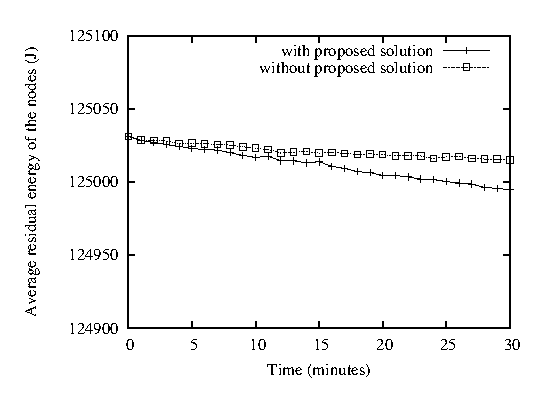
\includegraphics[width=.96\linewidth]{\chapterfig/mean.eps}
    \caption{Average residual energy of the nodes (excluding \ch)}\label{se:fig:mean}
\end{figure}
Average residual energy per minute in the batteries of the nodes is displayed on \figurename~\ref{se:fig:mean}.
Increasing values at $t=11$~minutes and $t=15$~minutes with the use of the proposed solution traduce the recovery effect of the batteries.
As expected, our proposal causes an increased global energy consumption.
This is due, of course, to the new \vn role.
\vns have to wake up periodically to send requests to neighbor \cns and to wait for an answer: this is energy-consuming.
The estimated overhead for our solution appears on \figurename~\ref{se:fig:overhead}.
\begin{figure}[ht]
    \centering
    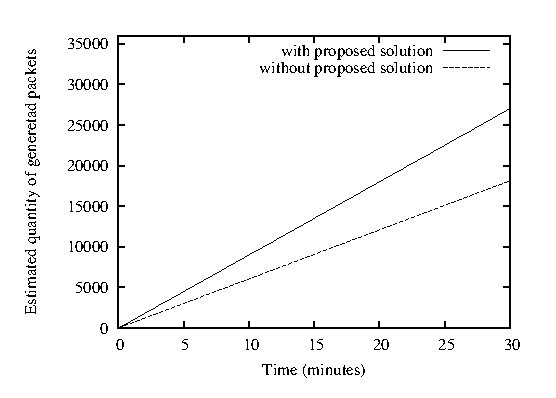
\includegraphics[width=.96\linewidth]{\chapterfig/overhead.eps}
    \caption{Estimated number of generated packets during the simulation}\label{se:fig:overhead}
\end{figure}

%%%%%%%%%%%%%%%%%%%%%%%%%%%%%%%%%%%%%%%%%%%%%%%%%%%%%%%%%%%%%%%%%%%%%%%%%%%%%%%
%Along with overall complexity, overhead is also increased.
%Both those factors impact the nodes consumption.
%Note that we do not seek to decrease the comprehensive consumption of energy in the network; instead, we try to improve load balancing in order to keep alive as many nodes in the cluster as we can as time goes by.
Standard deviation of residual energy value in the nodes at each minute of the simulation is presented on \figurename~\ref{se:fig:stddev}.
\begin{figure}[ht]
    \centering
    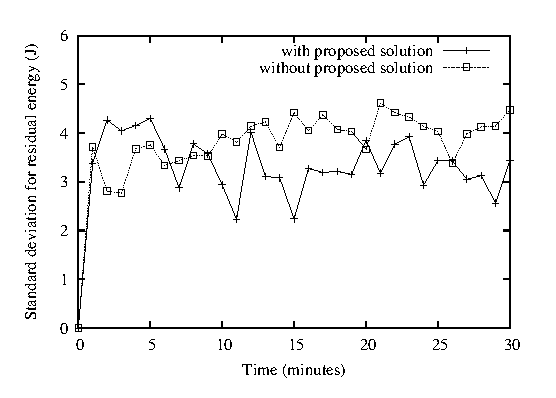
\includegraphics[width=.96\linewidth]{\chapterfig/stddev.eps}
    \caption{Standard deviation for residual energy of the nodes}\label{se:fig:stddev}
\end{figure}
During the first minutes of simulation, our solution creates a higher disproportion in load balancing due to the introduction of \vns (there are more nodes assuming demanding functions).
But after the seven first minutes or so, the standard deviation with our method falls below the standard deviation of previous method.
This is the consequence of a better load repartition over the nodes with our solution.
The difference between standard deviation with and without our simulation may look small: this is due to the model of the simulation we implemented.
Given that we have a good pseudo-random numbers generator, when the number of elections get high, all nodes will roughly assume \cn role the same number of times in simulation \emph{not} using our solution.
As sensing nodes all have the same activity, a correct repartition of the \cn roles over the time leads to a good energy balance.
But in a situation where sensing nodes have different activity levels ---~for instance, if there is an area in the cluster when measured events occur much more often than in the other parts of the cluster~--- the consumption would not be equilibrated between all the nodes with the previous method; whereas our solution would deal well with this case, since \cns are elected according to residual energy.
Thus simulations show that the use of \vns leads to a higher energy consumption, but electing \cns on residual energy provides a better load repartition in the cluster.
